\documentclass{article}

\usepackage[letterpaper,portrait,margin=1in]{geometry}

\usepackage{amsmath, amsfonts, amsthm, amssymb}
\usepackage{graphicx, float}
\usepackage{mathtools}
\usepackage{siunitx}
\usepackage{titlesec}
\usepackage{interval}
\usepackage{titling}
\usepackage{multicol}

\intervalconfig {
	soft open fences
}

\usepackage{tikz}
\usetikzlibrary{positioning}
\usetikzlibrary{angles,quotes}

\newtheorem*{theorem*}{Theorem}

%opening
\title{Problem Set \#33, Part 2}
\author{Jayden Li}
\date{December 8, 2023}

\begin{document}

\newgeometry{top=0.4in,bottom=1in,right=1in,left=1in}

\linespread{1.25}
\fontsize{12pt}{12pt}\selectfont

\title{Problem Set \#34}
\maketitle

\section*{Problem 8}
\begin{itemize}
	\item[(e)]
	\begin{align*}
		y=\arccos\left(\frac{x-3}{2x-1}\right)
	\end{align*}
	\begin{minipage}[t]{.45\textwidth}
	\begin{align*}
		\frac{x-3}{2x-1}&\geq-1 \\
		\frac{x-3}{2x-1}+\frac{2x-1}{2x-1}&\geq0 \\
		\frac{3x-4}{2x-1}&\geq0 \\
		\\
		2x-1&=0 \\
		x&=\frac{1}{2} \\
		\\
		3x-4&=0 \\
		x&=\frac{4}{3} \\
	\end{align*}
	\centering
	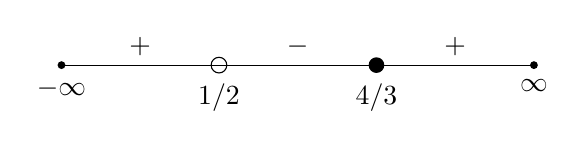
\begin{tikzpicture}	
		\draw
		(0,0) node[circle,fill,inner sep=1pt,label=below:$-\infty$](a){}
	 -- (2,0) node[circle,draw,inner sep=2pt,label=below:$1/2$](b){} node[midway,above]{$+$}
	 -- (4,0) node[circle,fill,inner sep=2pt,label=below:$4/3$](c){}node[midway,above]{$-$}
	 -- (6,0) node[circle,fill,inner sep=1pt,label=below:$\infty$](d){} node[midway,above]{$+$};
	\end{tikzpicture}
	\[
		x\in
		\interval[scaled,open left,open right]{-\infty}{\frac{1}{2}}\cup
		\interval[scaled,open right]{\frac{4}{3}}{\infty}
	\]
	\end{minipage}
	\begin{minipage}[t]{.45\textwidth}
	\begin{align*}
		\frac{x-3}{2x-1}&\leq1 \\
		\frac{x-3}{2x-1}-\frac{2x-1}{2x-1}&\leq0 \\
		\frac{-x-2}{2x-1}&\leq0 \\
		\\
		2x-1&=0 \\
		x&=\frac{1}{2} \\
		\\
		-x-2&=0 \\
		x&=-2 \\
	\end{align*}
	\centering
	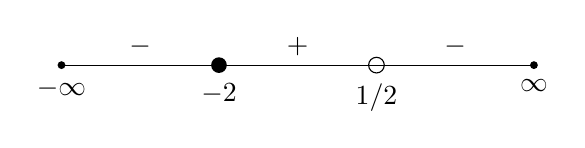
\begin{tikzpicture}	
		\draw
		(0,0) node[circle,fill,inner sep=1pt,label=below:$-\infty$](a){}
	 -- (2,0) node[circle,fill,inner sep=2pt,label=below:$-2$](b){} node[midway,above]{$-$}
	 -- (4,0) node[circle,draw,inner sep=2pt,label=below:$1/2$](c){} node[midway,above]{$+$}
	 -- (6,0) node[circle,fill,inner sep=1pt,label=below:$\infty$](d){} node[midway,above]{$-$};
	\end{tikzpicture}
	\[
		x\in
		\interval[scaled,open left]{-\infty}{-2}\cup
		\interval[scaled,open left,open right]{\frac{1}{2}}{\infty}
	\] \\
	\end{minipage}
	\begin{gather*}
		\\
		x\in
		\left(\interval[scaled,open left,open right]{-\infty}{\frac{1}{2}}\cup
		\interval[scaled,open right]{\frac{4}{3}}{\infty}\right)
		\cap\left(\interval[scaled,open left]{-\infty}{-2}\cup
		\interval[scaled,open left,open right]{\frac{1}{2}}{\infty}\right) \\
		\boxed{x\in
		\interval[scaled,open left]{-\infty}{-2}\cup
		\interval[scaled,open right]{\frac{4}{3}}{\infty}} \\
	\end{gather*}
\end{itemize}

\pagebreak

\newgeometry{top=0.75in,bottom=1in,right=0.5in,left=0.5in}

\section*{Problem 9}
\begin{theorem*}$
	\arcsin x-\arcsin y=
	\arcsin\left(x\sqrt{1-y^2}-y\sqrt{1-x^2}\right)
$\end{theorem*}
	
\begin{proof}
	\begin{center}
	\begin{minipage}[t]{.45\textwidth}
	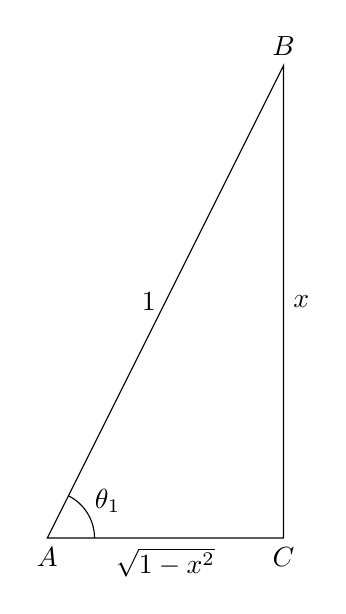
\begin{tikzpicture}[
		baseline=(current bounding box.north),
		ang/.style={draw, angle eccentricity=1.5,angle radius=0.6cm}
	]	
		\draw 
		(0,0) coordinate[label=below:{$A$}](A)
	 -- (3,0) coordinate[label=below:{$C$}](C) node[midway,below]{$\sqrt{1-x^2}$}
	 -- (3,6) coordinate[label=above:{$B$}](B) node[midway,right]{$x$}
	 -- cycle node[midway,above,left]{$1$}
	 	pic["$\theta_1$",ang]{angle=C--A--B};
	\end{tikzpicture}
	$\begin{aligned}[t]
		\\
		\text{Let }\theta_1&=\arcsin x \\
		\sin\theta_1&=\sin\left(\arcsin x\right) \\
		\frac{\text{opp}}{\text{hyp}}&=x \\
		\frac{BC}{AB}&=x \\
		\text{Let }BC&=x,\,AB=1 \\
		AC&=\sqrt{1-x^2} \\
		\\
		\sin\theta_1&=x \\
		\cos\theta_1&=\sqrt{1-x^2} \\
	\end{aligned}$
	\end{minipage}
	\begin{minipage}[t]{.45\textwidth}
	\begin{tikzpicture}[
		baseline=(current bounding box.north),
		ang/.style={draw, angle eccentricity=1.5,angle radius=0.6cm}
	]	
		\draw 
		(0,0) coordinate[label=below:{$D$}](D)
	 -- (3,0) coordinate[label=below:{$F$}](F) node[midway,below]{$\sqrt{1-y^2}$}
	 -- (3,6) coordinate[label=above:{$E$}](E) node[midway,right]{$y$}
	 -- cycle node[midway,above,left]{$1$}
	 	pic["$\theta_2$",ang]{angle=C--A--B};
	\end{tikzpicture}
	$\begin{aligned}[t]
		\\
		\text{Let }\theta_2&=\arcsin y \\
		\sin\theta_2&=\sin\left(\arcsin y\right) \\
		\frac{\text{opp}}{\text{hyp}}&=y \\
		\frac{EF}{DE}&=y \\
		\text{Let }EF&=y,\,DE=1 \\
		DF&=\sqrt{1-y^2} \\
		\\
		\sin\theta_2&=y \\
		\cos\theta_2&=\sqrt{1-y^2} \\
	\end{aligned}$
	\end{minipage}
	\end{center}

	\begin{align*}
		\text{RHS: }&\arcsin\left(x\sqrt{1-y^2}-y\sqrt{1-x^2}\right) \\
		&=\arcsin\left(\sin\theta_1\cos\theta_2-\sin\theta_2\cos\theta_1\right) \\
		&=\arcsin\left(\sin\left(\theta_1-\theta_2\right)\right) \\
		&=\theta_1-\theta_2\ \\
		&=\arcsin x-\arcsin y
	\end{align*}
\end{proof}

\end{document}
